% !TEX root = paper.tex

\section {Results}
\label{sec:results}
This section presents final results of the extracted $v_2$ and $v_3$ as a function of $p_{\mathrm{T},trig}$ and the event-scale selections, and the extracted $v_2$ as a function of multiplicity. 

\subsection{$p_{\mathrm{T}}$ and Multiplicity dependence}

\begin{figure}[!th]
	\centering
	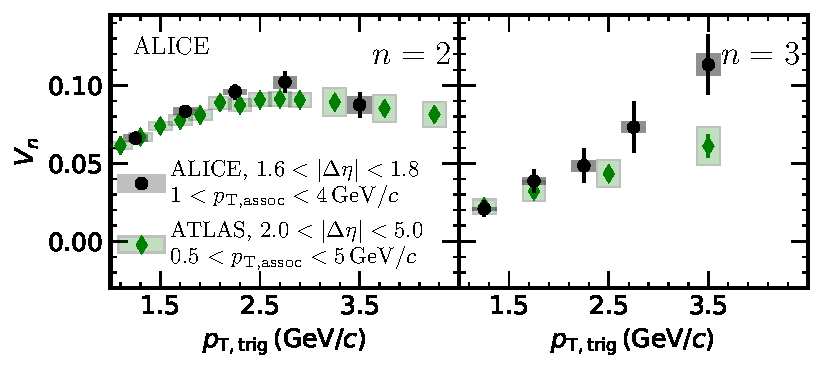
\includegraphics[width=0.9 \textwidth]{figures/Fig2_vn.pdf} 
	\caption{The magnitude of $v_2$ (left) and $v_3$ (right) as a function of $p_\mathrm{T}$ for ALICE (black) and ATLAS (blue). }
	\label{fig:vn}
\end{figure}

The extracted $v_2$ and $v_3$ are shown as a function of $p_{\mathrm{T},trig}$ (GeV/c) in Fig.~\ref{fig:vn}. These results are obtained from the 13 TeV pp template fits for the high multiplicity class of $0-0.1\%$ at a large $\Delta\eta$ range of $1.6<|\Delta\eta|<1.8$ and an associated particle $p_{\mathrm{T},assoc}$ acceptance of $1<p_{\mathrm{T},assoc}<4$ GeV/c. The ATLAS experiment used the same method to extract $v_2$ and $v_3$ in~\cite{Aaboud:2016yar}, hence their results are also shown in Fig.~\ref{fig:vn}, with the same system energy and multiplicity class, for comparison. The large $\Delta\eta$ range for the ATLAS results is $2.0<|\Delta\eta|<5.0$ and the associated particle $p_{\mathrm{T},assoc}$ acceptance is $0.5<p_{\mathrm{T},assoc}<5$ GeV/c. When comparing ALICE to ATLAS results, they seem to agree for lower $p_{\mathrm{T},trig}$ but not for higher. However, one should note that ATLAS and ALICE has different multiplicity definitions, hence this is not an apple to apple comparison. 


\begin{figure}[!th]
	\centering
	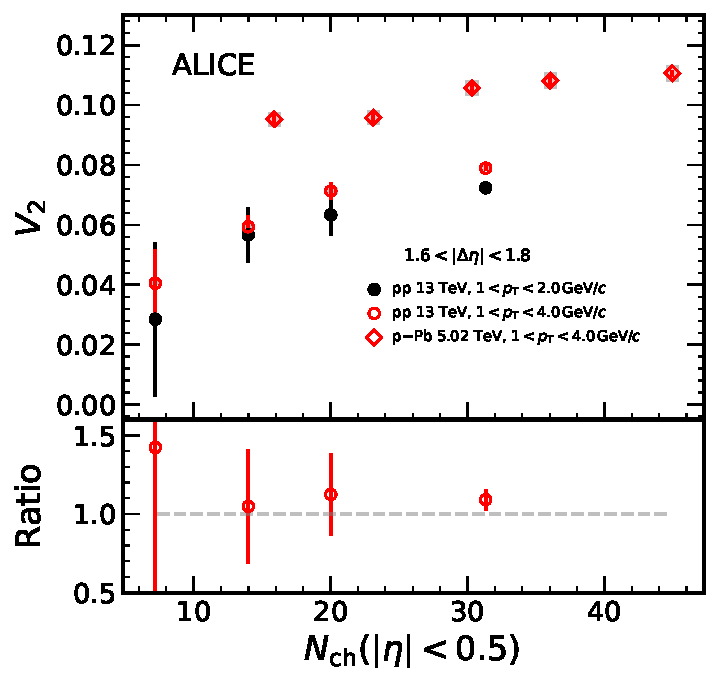
\includegraphics[width=0.8 \textwidth]{figures/Fig6_v2Mult_allSystemsComp2.pdf} 
	\caption{The $v_2$ magnitude for two different system sizes, pp and p-Pb, as a function of multiplicity. Additionally, pp collisions for two different $p_\mathrm{T}$ bins, $1.0<p_\mathrm{T}<2.0$ GeV/c and $1.0<p_\mathrm{T}<4.0$ GeV/c, are presented. The the system sizes are differentiated with two different markers, circles and rhombuses, for pp and p-Pb respectively. The $p_\mathrm{T}$ bins, are differentiated with different colored markers; black for the $1.0<p_\mathrm{T}<2.0$ GeV/c bin and red for the $1.0<p_\mathrm{T}<4.0$ GeV/c bin. In the ratio the statistical and systematic errors are combined in quadrature.} 
	\label{fig:v2mult}
\end{figure}

In Fig.\ref{fig:v2mult} the magnitude of $v_2$ as a function of multiplicity is presented for both pp and p-Pb collision systems, at 13 and 5.02 TeV respectively. As in Fig.~\ref{fig:vn}, the large $\Delta\eta$ range is at $1.6<|\Delta\eta|<1.8$ and the associated particle $p_{\mathrm{T},assoc}$ acceptance is $1<p_{\mathrm{T},assoc}<4$ GeV/c for both collision systems. Additionally, pp collisions at 13 TeV with an associated particle $p_{\mathrm{T},assoc}$ acceptance of $1<p_{\mathrm{T},assoc}<2$ GeV/c is presented. Conclusions for the figure is that the magnitude of $v_2$ is clearly larger in p-Pb collisions, which was expected due to the larger system size. For the two different $p_\mathrm{T}$ bins presented for the pp collisions, the $v_2$ for the $1.0<p_\mathrm{T}<4.0$ GeV/c bin is larger than $v_2$ for the $1.0<p_\mathrm{T}<2.0$ GeV/c bin, also as expected.

\subsection{Event-scale dependence}
\begin{figure}[!th]
	\centering
	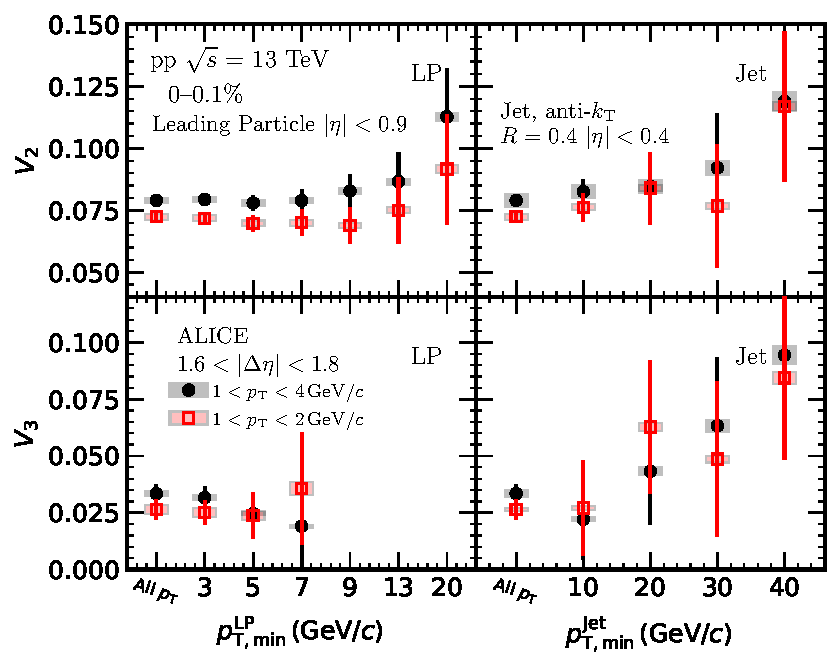
\includegraphics[width=0.8 \textwidth]{figures/Fig4_vn_LP.pdf}
	\caption{The magnitude of $v_2$ (top) and $v_3$ (bottom) as a function of minimum $p_{\mathrm{T}}$ for leading particle (left) and jet (right).}
	\label{fig:LPjet23}
\end{figure}

Figure~\ref{fig:LPjet23} presents the extracted magnitude of $v_2$ and $v_3$ as a function of two different event scale selections; $p_{\mathrm{T,min}}^{\mathrm{LP}}$ and $p_{\mathrm{T,min}}^{\mathrm{Jet}}$ for the Leading Particle track and reconstructed jet, respectively. Both event scale results are obtained from pp collisions at 13 TeV for the multiplicity class of $0-0.1\%$. The associated particle $p_{\mathrm{T},assoc}$ acceptance is $1<p_{\mathrm{T},assoc}<2$ GeV/c and the large $\Delta\eta$ range at $1.6<|\Delta\eta|<1.8$. In these results the leading particle is required to be within $|\eta|<0.9$ and the jets are reconstructed using the anti$-k_\mathrm{T}$ algorithm with R=0.4 and are required to be within $|\eta|<0.4$. Both $v_2$ and$v_3$ show weakly increasing or consistent trend with increasing event-scale selection, with a larger increase of $v_n$ magnitude for the event selection of jets. 